% Diapositivas de la sustentación - Grupo 6 (máximo 12 láminas, 10 a 12 minutos)
% Compila con XeLaTeX o pdfLaTeX.
\documentclass[11pt,aspectratio=169]{beamer}
\usetheme[progressbar=frametitle,numbering=fraction]{metropolis}
\usepackage{iftex}
\ifXeTeX
  \usepackage{polyglossia}\setmainlanguage{spanish}
\else
  \usepackage[utf8]{inputenc}\usepackage[T1]{fontenc}
  \usepackage[spanish,es-noshorthands,es-nodecimaldot]{babel}
\fi
\usepackage{amsmath,amssymb,booktabs,tikz}
\usetikzlibrary{arrows.meta,positioning}
\definecolor{azul}{HTML}{2A6FB0}
\definecolor{gris}{HTML}{5F6B76}
\setbeamercolor{frametitle}{bg=azul}
\setbeamercolor{progress bar}{fg=azul}
\setbeamercolor{alerted text}{fg=azul}
\newcommand{\Th}{\Theta}
% Generado por informe/generar_valores.py a partir de resultados/*.json. No editar a mano.
\newcommand{\cUnoPendUni}{1{,}22}
\newcommand{\cUnoPendAgr}{1{,}22}
\newcommand{\cUnoPendVer}{1{,}24}
\newcommand{\cUnoPendFB}{1{,}89}
\newcommand{\cUnoPendTeo}{1{,}11}
\newcommand{\cUnoBajoMin}{1{,}13}
\newcommand{\cUnoBajoMax}{1{,}16}
\newcommand{\cUnoAltoMin}{1{,}28}
\newcommand{\cUnoAltoMax}{1{,}30}
\newcommand{\cUnoPendComb}{1{,}11}
\newcommand{\cUnoPendDist}{1{,}01}
\newcommand{\cUnoMaxVecinos}{2}
\newcommand{\cUnoSpeedup}{47{,}0}
\newcommand{\cUnoCruce}{64}
\newcommand{\cUnoCombIni}{1{,}80}
\newcommand{\cUnoCombFin}{1{,}89}
\newcommand{\cDosN}{1\,048\,576}
\newcommand{\cDosCosto}{2\,621\,434}
\newcommand{\cDosCota}{3\,145\,728}
\newcommand{\cDosMaxRazon}{2{,}99999}
\newcommand{\cDosMinRazon}{1{,}94}
\newcommand{\cDosBancoMin}{2}
\newcommand{\cDosDuplic}{18}
\newcommand{\cDosPendT}{1{,}12}
\newcommand{\cDosPendBajo}{1{,}13}
\newcommand{\cDosPendAlto}{1{,}16}
\newcommand{\cDosUsIni}{2{,}3}
\newcommand{\cDosUsFin}{5{,}0}
\newcommand{\cDosPendN}{1{,}99}
\newcommand{\cDosPendTabla}{2{,}00}
\newcommand{\cDosPendDensa}{3{,}00}
\newcommand{\cDosBytesVox}{410}
\newcommand{\cDosMiBTabla}{48}
\newcommand{\cDosMiBDensa}{64}
\newcommand{\cDosLrMax}{256}
\newcommand{\cTresFact}{321}
\newcommand{\cTresIguales}{321}
\newcommand{\cTresInst}{2000}
\newcommand{\cTresInfact}{1679}
\newcommand{\cTresInfactOk}{1679}
\newcommand{\cTresLargo}{216}
\newcommand{\cTresExceso}{4}
\newcommand{\cTresEjOpt}{4}
\newcommand{\cTresEjLargo}{8}
\newcommand{\cTresPendTotal}{1{,}30}
\newcommand{\cTresPendBarrido}{1{,}11}
\newcommand{\cTresPendTotalBajo}{1{,}17}
\newcommand{\cTresPendBarridoBajo}{0{,}88}
\newcommand{\cTresPendComp}{1{,}11}
\newcommand{\cTresPendTeo}{1{,}10}
\newcommand{\cTresFracBarrido}{7{,}9}
\newcommand{\cCuatroFactor}{1{,}24}
\newcommand{\cCuatroK}{7}
\newcommand{\cCuatroSinMed}{50\,606}
\newcommand{\cCuatroSinMax}{3\,000\,000}
\newcommand{\cCuatroCortes}{2}
\newcommand{\cCuatroConMed}{16}
\newcommand{\cCuatroBfsMed}{38}
\newcommand{\cCuatroRazon}{3\,893}
\newcommand{\cCuatroTSin}{0{,}06}
\newcommand{\cCuatroTCon}{0{,}09}
\newcommand{\cCuatroPendBfs}{1{,}02}
\newcommand{\cCuatroPendPoda}{2{,}36}
\newcommand{\cCuatroPodaK}{32}
\newcommand{\cCuatroPodaMed}{18\,214}
\newcommand{\cCuatroPodaMax}{3\,000\,000}
\newcommand{\cCuatroPodaCortes}{2}
\newcommand{\cCuatroParqLong}{17}
\newcommand{\cCuatroParqCon}{124}
\newcommand{\cCuatroParqSin}{7\,075}
\newcommand{\cCuatroParqBfs}{68}
\newcommand{\cCincoExactaCarga}{sí}
\newcommand{\cCincoExactaPunto}{sí}
\newcommand{\cCincoRangos}{sí}
\newcommand{\cCincoPendT}{1{,}01}
\newcommand{\cCincoPendES}{1{,}00}
\newcommand{\cCincoNMax}{1\,000\,000}
\newcommand{\cCincoMMax}{50\,000}
\newcommand{\cCincoMB}{294}
\newcommand{\cCincoH}{3}
\newcommand{\cCincoRecorrido}{5\,883}
\newcommand{\cCincoInsCienN}{2\,000}
\newcommand{\cCincoInsCienLect}{3{,}00}
\newcommand{\cCincoInsCienEscr}{1{,}57}
\newcommand{\cCincoInsCienDiv}{28}
\newcommand{\cCincoInsCienExactas}{2\,000}
\newcommand{\cCincoInsCienH}{3}
\newcommand{\cCincoInsSetentaN}{2\,000}
\newcommand{\cCincoInsSetentaLect}{3{,}00}
\newcommand{\cCincoInsSetentaEscr}{1{,}00}
\newcommand{\cCincoInsSetentaDiv}{0}
\newcommand{\cCincoInsSetentaExactas}{2\,000}
\newcommand{\cCincoInsSetentaH}{3}
\newcommand{\cSeisGrafos}{400}
\newcommand{\cSeisCumplen}{400}
\newcommand{\cSeisMediaCalles}{1{,}88}
\newcommand{\cSeisMediaAleat}{1{,}56}
\newcommand{\cSeisMax}{2{,}00}
\newcommand{\cSeisMin}{1{,}17}
\newcommand{\cSeisGradoMax}{1{,}04}
\newcommand{\cSeisPendT}{0{,}97}
\newcommand{\cSeisFactorFB}{2{,}08}
\newcommand{\cSeisAjC}{16}
\newcommand{\cSeisAjOpt}{8}
\newcommand{\cSeisFBVmax}{20}
\newcommand{\cSeisFBTmax}{0{,}33}


\title{Percepción y navegación de un vehículo autónomo urbano}
\subtitle{Proyecto Final Integrador -- Análisis de Algoritmos (SIST0175) -- Grupo 6}
\author{Santiago Felipe Fajardo \and Sebastián Páez Castañeda \and Johan Sebastián Acuña}
\institute{Universidad Sergio Arboleda -- Docente: Juan David Rodríguez Martínez}
\date{Noviembre de 2026}

\begin{document}
\maketitle

% 2 ------------------------------------------------------------------
\begin{frame}{El caso y los seis componentes}
\centering
\resizebox{0.92\textwidth}{!}{%
\begin{tikzpicture}[font=\footnotesize,
  c/.style={draw=azul,rounded corners=3pt,align=center,minimum width=3.6cm,minimum height=0.95cm,line width=0.7pt},
  d/.style={draw=gris,fill=gray!8,rounded corners=2pt,align=center,minimum width=2.8cm,minimum height=0.7cm},
  f/.style={-{Stealth[length=2mm]},gris}]
  \node[d] (n) at (-2,0) {Nube LiDAR 3D};
  \node[d] (t) at (4,0) {Trayectoria y sensores};
  \node[d] (l) at (8.4,0) {Telemetría};
  \node[c] (c1) at (-4,-1.45) {\textbf{C1} Par más cercano\\D\&V};
  \node[c] (c2) at (0,-1.45) {\textbf{C2} Mapa de vóxeles\\tabla hash};
  \node[c] (c3) at (4,-1.45) {\textbf{C3} Cobertura de $[0,L]$\\voraz};
  \node[c] (c5) at (8.4,-1.45) {\textbf{C5} Árbol B+\\en disco};
  \node[c] (c4) at (0,-3.0) {\textbf{C4} Maniobra\\backtracking / BFS};
  \node[c] (c6) at (4,-3.0) {\textbf{C6} Sensores en cruces\\2-aproximación};
  \draw[f] (n.south) -- ++(0,-0.25) -| (c1.north); \draw[f] (n.south) -- (c2.north);
  \draw[f] (t) -- (c3); \draw[f] (l) -- (c5); \draw[f] (c2) -- (c4); \draw[f] (c3) -- (c6);
\end{tikzpicture}}

\medskip
\small Datos sintéticos con semilla fija (6) \quad·\quad 44 pruebas pytest \quad·\quad sin \texttt{sorted}, \texttt{heapq} ni \texttt{networkx} en el núcleo
\end{frame}

% 3 ------------------------------------------------------------------
\begin{frame}{C1 -- Par más cercano por divide y vencerás}
\begin{columns}[T]
\column{0.45\textwidth}
\small
\begin{itemize}
\item Ordenar por $x$ una vez; dividir; mezclar por $y$; revisar la franja $|x-x_m|<d$
\item Lema: $\le7$ vecinos por punto (8 cuadros de lado $d/2$)
\item $T(n)=2T(n/2)+\Th(n)$\\$a=2$, $b=2$, $f(n)=\Th(n^{\log_2 2})$\\\alert{caso 2} $\Rightarrow\Th(n\log n)$
\item Medido: pendiente $\cUnoBajoMin$--$\cUnoBajoMax$ (ref. $\cUnoPendTeo$); conteo $\cUnoPendComb$; FB $\cUnoPendFB$
\item $\cUnoSpeedup\times$ más rápido que fuerza bruta en $n=4096$
\end{itemize}
\column{0.55\textwidth}
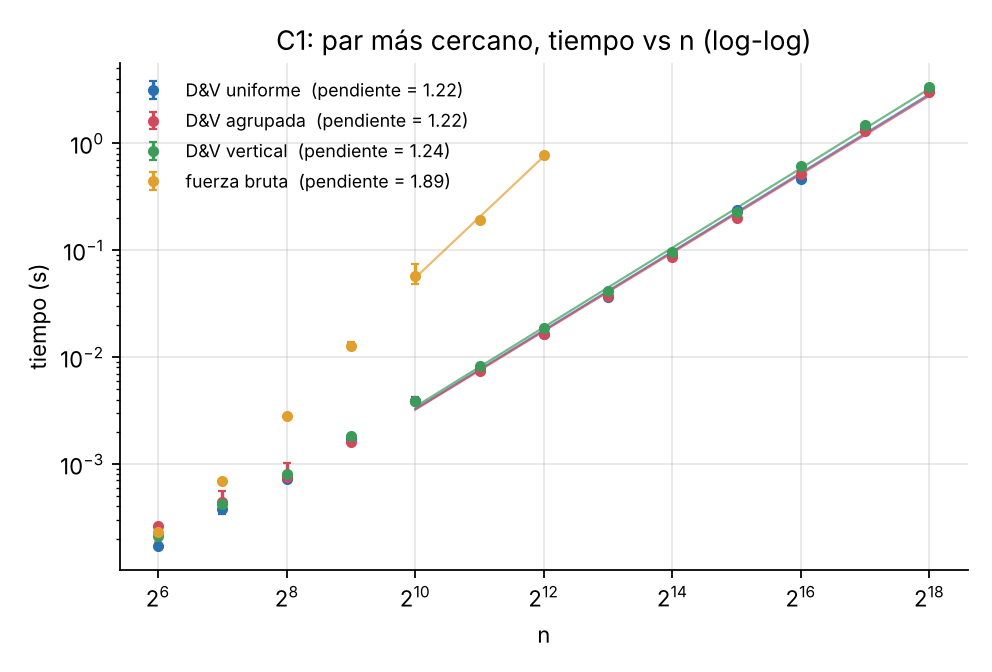
\includegraphics[width=\linewidth]{figuras/c1_loglog.png}
\end{columns}
\end{frame}

% 4 ------------------------------------------------------------------
\begin{frame}{C2 -- Mapa de vóxeles: método contable}
\small
\begin{columns}[T]
\column{0.4\textwidth}
\begin{itemize}
\item Solo vóxeles ocupados; se duplica al pasar $\alpha=3/4$
\item $\hat c=3$: colocarse, moverse, mover una clave vieja
\item Entre duplicaciones entran $t$ claves ($2t$ créditos) y se mueven $2t$: banco $\ge0$
\item $C(n)=\cDosCosto\le3n=\cDosCota$
\item Espacio: tabla $\cDosPendTabla$ vs rejilla $\cDosPendDensa$ (pendiente en $L/r$)
\end{itemize}
\column{0.6\textwidth}
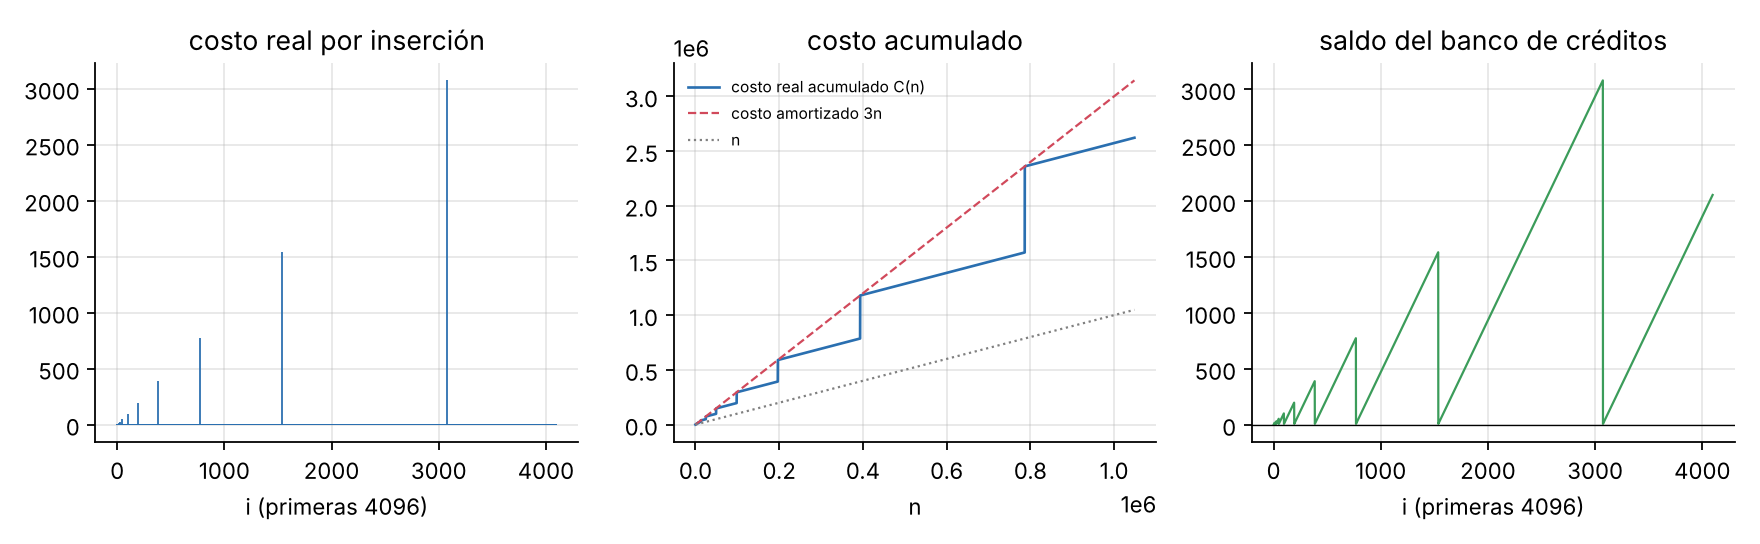
\includegraphics[width=\linewidth,height=0.36\textheight,keepaspectratio]{figuras/c2_metodo_contable.png}\\
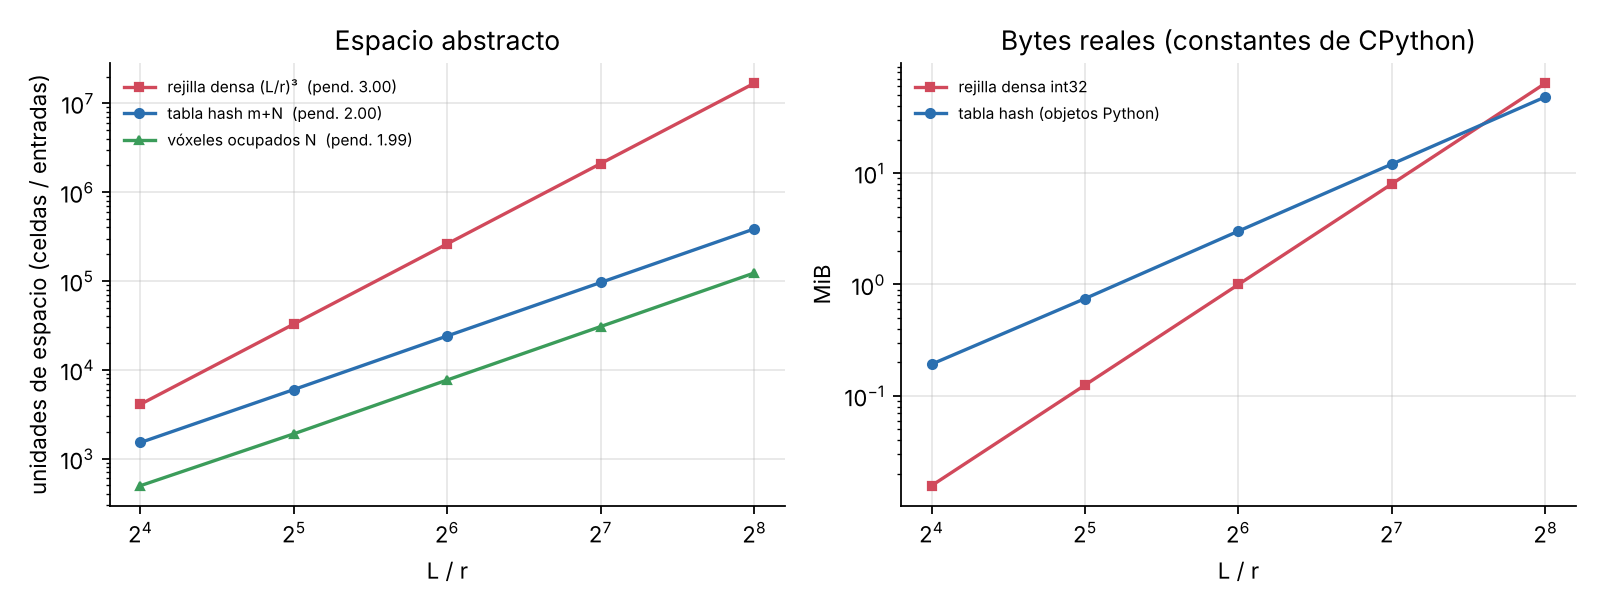
\includegraphics[width=0.8\linewidth,height=0.36\textheight,keepaspectratio]{figuras/c2_espacio.png}
\end{columns}
\end{frame}

% 5 ------------------------------------------------------------------
\begin{frame}{C3 -- Voraz: cobertura mínima de la trayectoria}
\begin{columns}[T]
\column{0.5\textwidth}
\small
\textbf{Regla}: de los tramos con $a\le x$, el de mayor $b$.

\textbf{Intercambio}: un óptimo tiene $o$ con $a_o\le x$; como $b_g\ge b_o$, cambiar $o$ por $g$ sigue
cubriendo $\Rightarrow$ hay un óptimo con $g$; más subestructura e inducción.

\textbf{Contraejemplo}: ``más largo primero'' con $[0,5],[5,10],[2,8]$ usa 3 (óptimo 2).

\medskip
\begin{tabular}{lr}
\toprule
Voraz $=$ óptimo & \alert{$\cTresIguales$/$\cTresFact$} \\
Infactibles detectadas & $\cTresInfactOk$/$\cTresInfact$ \\
``Más largo'' subóptimo & $\cTresLargo$ \\
Pendiente ($2^{10}..2^{14}$) & $\cTresPendTotalBajo$ \\
\bottomrule
\end{tabular}
\column{0.5\textwidth}
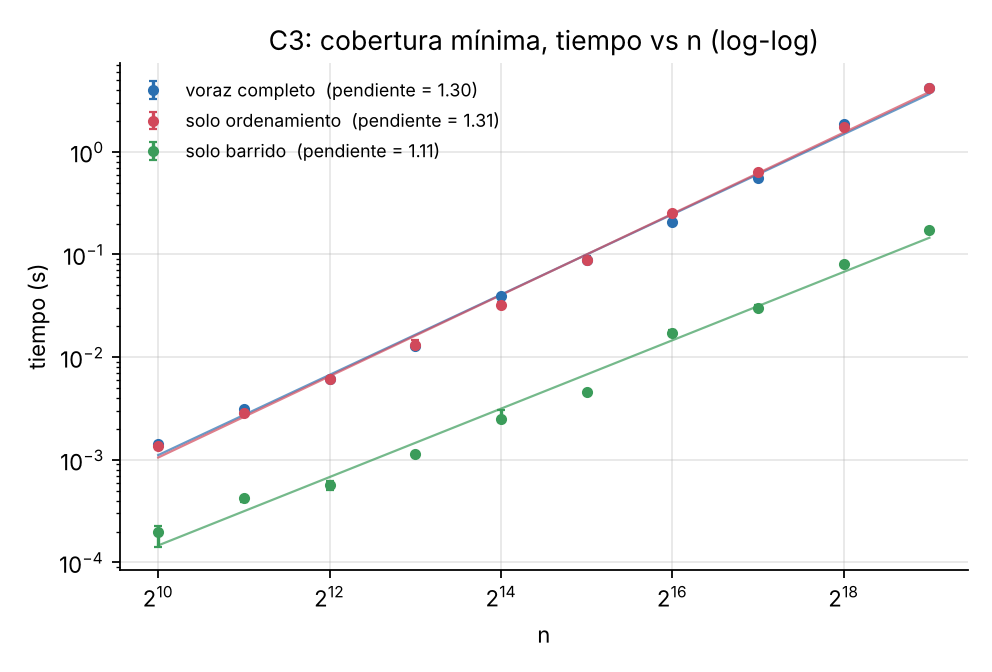
\includegraphics[width=\linewidth]{figuras/c3_loglog.png}
\end{columns}
\end{frame}

% 6 ------------------------------------------------------------------
\begin{frame}{C4 -- Maniobra: backtracking, poda Manhattan y BFS}
\begin{columns}[T]
\column{0.42\textwidth}
\small
\begin{itemize}
\item Árbol de búsqueda: caminos simples, $O(3^V)$
\item Poda: $g+h(v)\ge mejor$, con $h$ = Manhattan $\le$ distancia real $\Rightarrow$ no pierde el óptimo
\item Mejor caso con poda: $\Th(d)$
\item BFS: $\Th(V)$, pendiente $\cCuatroPendBfs$
\item $\cCuatroK\times\cCuatroK$: \alert{$\cCuatroSinMed$} nodos sin poda vs \alert{$\cCuatroConMed$} con poda
\item La poda no cambia el peor caso
\end{itemize}
\column{0.58\textwidth}
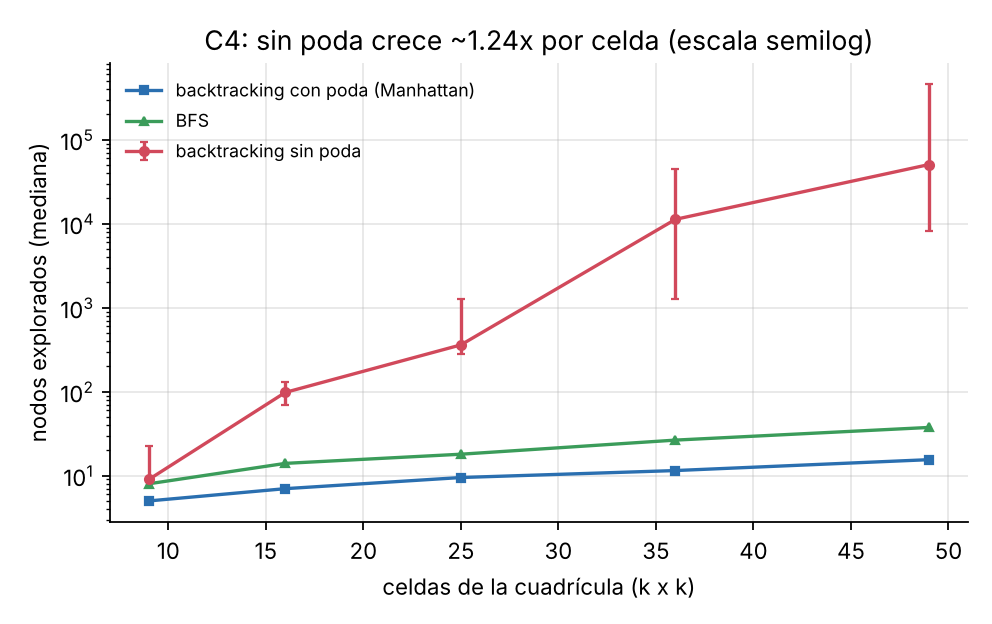
\includegraphics[width=\linewidth]{figuras/c4_nodos_pequenas.png}
\end{columns}
\end{frame}

% 7 ------------------------------------------------------------------
\begin{frame}{C5 -- Árbol B+ en disco: E/S predichas vs contadas}
\begin{columns}[T]
\column{0.45\textwidth}
\small
$B=170$ reg/hoja, $F=341$, $M=N/20$, \texttt{DiscoSimulado}
\[
\begin{aligned}
\text{carga} &: 1+\lceil N/B\rceil \text{ L},\ \textstyle L+\sum I_j+1 \text{ E}\\
\text{punto} &: h \text{ L}\\
\text{rango} &: [h-1,\,h]+\lceil k/b\rceil \text{ L}\\
\text{inserción} &: h \text{ L},\ 1+2s+[\text{raíz}] \text{ E}
\end{aligned}
\]
\begin{itemize}
\item Carga y punto exactos en los 6 tamaños
\item 300 rangos dentro de la fórmula
\item $N=\cCincoNMax$: $\cCincoH$ lecturas vs $\cCincoRecorrido$ recorriendo todo
\end{itemize}
\column{0.55\textwidth}
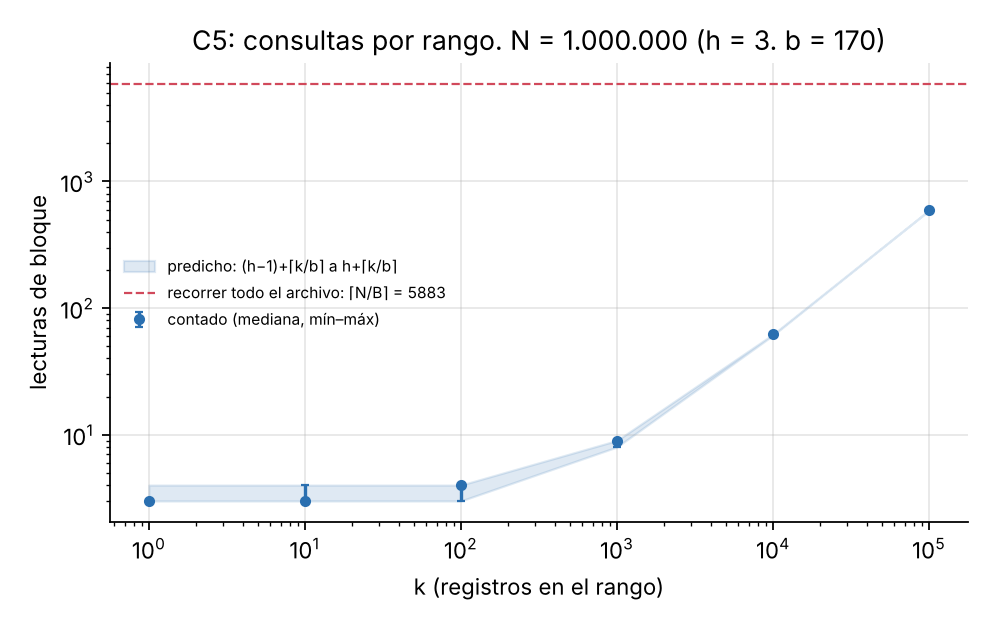
\includegraphics[width=\linewidth]{figuras/c5_rangos.png}
\end{columns}
\end{frame}

% 8 ------------------------------------------------------------------
\begin{frame}{C6 -- Sensores en intersecciones: 2-aproximación}
\begin{columns}[T]
\column{0.45\textwidth}
\small
\textbf{Algoritmo}: si $(u,v)$ no está cubierta, tomar $u$ y $v$ ($\Th(V+E)$).

\textbf{Prueba}: las aristas tomadas forman un emparejamiento $M$; todo óptimo toca cada una en un
vértice distinto $\Rightarrow OPT\ge|M|$, y $|C|=2|M|\le2\,OPT$.

\textbf{Ajustada}: aristas disjuntas, razón 2.

\medskip
$\cSeisCumplen$/$\cSeisGrafos$ grafos dentro de la cota\\
Razón media: calles $\cSeisMediaCalles$, aleatorios $\cSeisMediaAleat$\\
Pendiente del tiempo: $\cSeisPendT$
\column{0.55\textwidth}
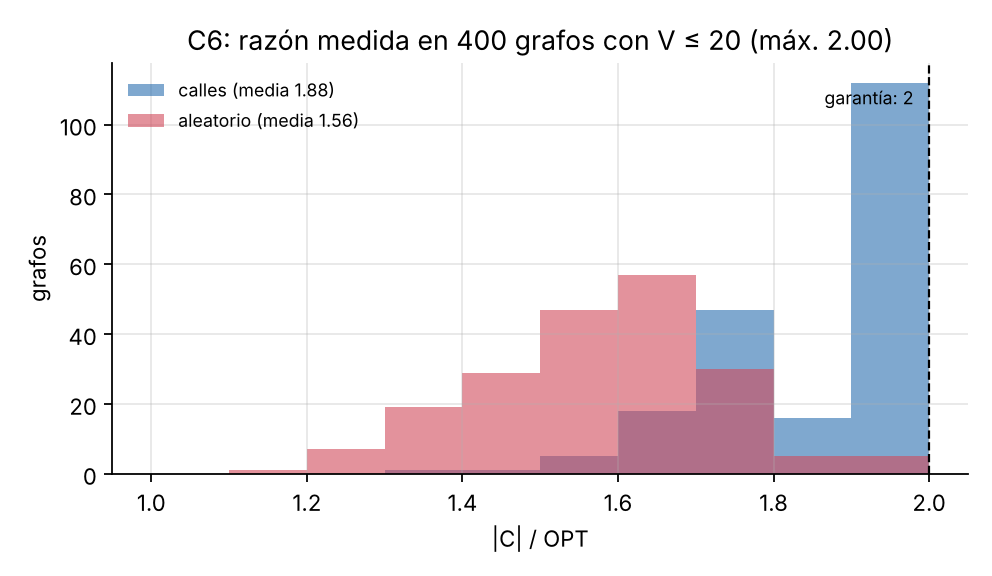
\includegraphics[width=\linewidth]{figuras/c6_razones.png}
\end{columns}
\end{frame}

% 9 ------------------------------------------------------------------
\begin{frame}{Validación: hipótesis frente a resultados}
\small
\centering
\begin{tabular}{lll}
\toprule
Hipótesis & Predicho & Medido \\
\midrule
C1 D\&V (tiempo, $2^{10}..2^{14}$) & $\approx\cUnoPendTeo$ & $\cUnoBajoMin$--$\cUnoBajoMax$ \\
C1 trabajo de combinación (conteo) & $\approx\cUnoPendTeo$ & $\cUnoPendComb$ \\
C2 costo acumulado & $\le3n$ & $\max C(n)/n=\cDosMaxRazon$ \\
C3 voraz $=$ óptimo & 100\,\% & $\cTresIguales$ de $\cTresFact$ \\
C4 sin poda & exponencial & $\times\cCuatroFactor$ por celda \\
C4 BFS & pendiente 1 & $\cCuatroPendBfs$ \\
C5 E/S carga y punto & exactas & exactas (\cCincoExactaCarga) \\
C6 razón & $\le2$ & máx. $\cSeisMax$, media $\cSeisMediaCalles$ \\
\bottomrule
\end{tabular}
\end{frame}

% 10 ------------------------------------------------------------------
\begin{frame}{Discusión: dónde no coincide y por qué}
\begin{enumerate}
\item \textbf{Caché}: desde $n\approx2^{14}$ los datos (objetos de Python de $\sim$100\,B) no caben en la L2
de 4\,MiB y las pendientes de tiempo suben (C1 $\cUnoAltoMax$, C3 $\cTresPendTotal$).
\item \textbf{$n\log n$ no tiene pendiente 1}: $1+1/\ln n\approx1{,}1$.
\item \textbf{Constantes}: $\approx\cDosBytesVox$\,B por vóxel; la tabla gana en bytes solo desde $L/r=\cDosLrMax$.
\item \textbf{Peor caso vs práctica}: $\le7$ vecinos $\to$ máximo $\cUnoMaxVecinos$; razón $\le2$ $\to$ media
$\cSeisMediaCalles$; la poda de C4 explota en cuadrículas grandes.
\item Lo que se \alert{cuenta} coincide con la teoría; C5 (modelo de memoria externa) es exacto.
\end{enumerate}
\end{frame}

% 12 ------------------------------------------------------------------
\begin{frame}{Conclusiones y reparto}
\small
\begin{itemize}
\item En C1 y C3 el $n\log n$ lo pone el ordenamiento/mezcla, no las distancias ni el barrido
\item Duplicar la tabla: $\Th(N)$ en una inserción pero $O(1)$ amortizado
\item La poda reduce órdenes de magnitud, pero no el peor caso exponencial
\item Contar bloques predice el costo exacto en disco
\item Una prueba corta garantiza la razón 2 en un problema NP-difícil
\end{itemize}
\medskip
\begin{tabular}{ll}
\toprule
Santiago Felipe Fajardo & C1 y C2 \\
Sebastián Páez Castañeda & C3 y C4 \\
Johan Sebastián Acuña & C5 y C6 \\
Todos & experimentos, informe y diapositivas \\
\bottomrule
\end{tabular}
\end{frame}

\end{document}
